% %%%%%%%%%%%%%%%%%%%%%%%%%%%%%%%%%%%%%%%%%%%%%%%%%%%%%%%%%%%%%%%%%%%%%
% %% Theory %%
% Analysis
% %%%%%%%%%%%%%%%%%%%%%%%%%%%%%%%%%%%%%%%%%%%%%%%%%%%%%%%%%%%%%%%%%%%%%

\section{Analysis of Reduction Cache Behavior}
\label{sec:theory:analysis}

We now study the \gls{redC} behavior when computing \acrshort{op} \acrshort{spmv}, starting with the simple case of \gls{PBanded} matrices with varying \gls{band} widths.
We then use the analytical model to analyse the \gls{redC} behavior, varying the out-of-\gls{band} density and the cache-size.
We show the benefit of storing the in- and out-of-\gls{band} of the matrix in separate regions of the cache, to achieve low memory traffic.

% %%%%%%%%%%%%%%%%%%%%%%%%%%%%%%%%%%%%%%%%%%%%%%%%%%%%%%%%%%%%%%%%%%%%%
\subsection{Behavior of a Perfect-Band in a Cache}
\label{sec:perfectband_vs_cache}

\begin{figure}[htbp]
    \centering
    \begin{subfigure}{0.49\linewidth}
        \centering
        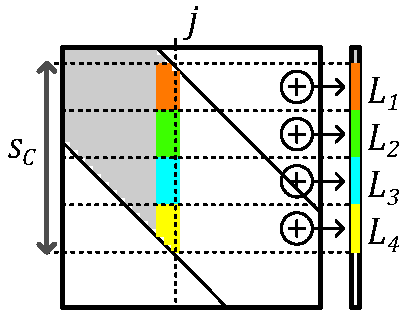
\includegraphics[width=\linewidth]{Chapter_Theory/Figures/PDF/PBrotationCase1_0.pdf}
        \caption{Column iteration $j$}
        \label{fig:theory:in_band_rotation_00}
    \end{subfigure}
    \hfill
    \begin{subfigure}{0.49\linewidth}
        \centering
        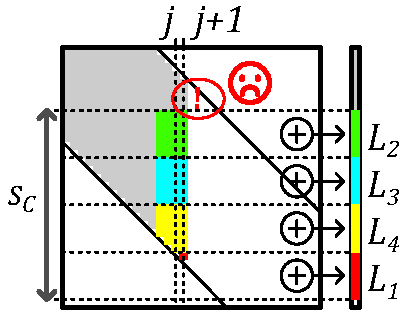
\includegraphics[width=\linewidth]{Chapter_Theory/Figures/PDF/PBrotationCase1_1.pdf}
        \caption{Column iteration $j+1$}
        \label{fig:theory:in_band_rotation_01}
    \end{subfigure}
    \caption{Example of the \Gls{eviction} Rotation in a Perfect \Gls{band} when the Cache is Undersized ($s_C < w_B + l - 1$) \note{redo? there is space, clarify where is c}}
    \label{fig:theory:in_band_rotation_case1}
\end{figure}

\begin{figure}[htbp]
    \centering
    \begin{subfigure}{0.49\linewidth}
        \centering
        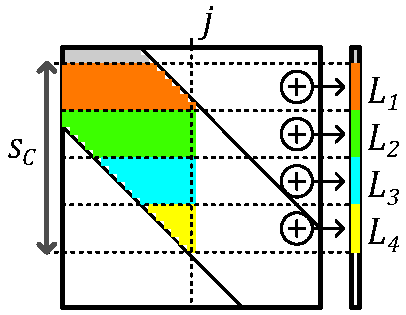
\includegraphics[width=\linewidth]{Chapter_Theory/Figures/PDF/PBrotationCase2_0.pdf}
        \caption{Column iteration $j$}
        \label{fig:theory:in_band_rotation_10}
    \end{subfigure}
    \hfill
    \begin{subfigure}{0.49\linewidth}
        \centering
        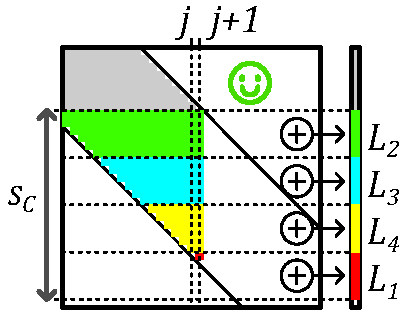
\includegraphics[width=\linewidth]{Chapter_Theory/Figures/PDF/PBrotationCase2_1.pdf}
        \caption{Column iteration $j+1$}
        \label{fig:theory:in_band_rotation_11}
    \end{subfigure}
    \caption{Example of the \Gls{eviction} Rotation in a Perfect \Gls{band} when the Cache is `Properly' Sized ($s_C = w_B + l - 1$)}
    \label{fig:theory:in_band_rotation_case2}
\end{figure}

In the previous chapter, we presented \acrlong{spdc} and a \gls{redC} baseline with a specific region (\acrshort{drc}) dedicated to storing the \gls{banded} region of the matrix.
We precised that the \gls{band} of the matrix is chosen depending on the \acrshort{drc} size.
In this section, we explain and precise this choice by analyzing the behavior of a \gls{redC} when processing an \acrshort{op} \acrshort{spmv} kernel with a \gls{PBanded} matrix.

We show that the \gls{redC} must be `properly' dimensioned with respect to the \gls{band} width of a \gls{PBanded} matrix, in order to avoid unnecessary \glspl{eviction}.
Indeed, if the cache is too small compared to the \gls{band}, \glspl{eviction} occur before the column iteration is over, leading to poor data-reuse for the next iteration.
To achieve high data-reuse, we show that the cache-size ($s_C$) and the \gls{band} width ($w_B$) must respect the relationship given in Equation~\ref{eq:theory:in_band_cond}.

\begin{equation}
    s_C \geqslant w_B + l - 1
    \label{eq:theory:in_band_cond}
\end{equation}

We consider two examples with a cache having four cache-lines ($L_1$ to $L_4$) with $l = 6$.
In Figure~\ref{fig:theory:in_band_rotation_case1}, we illustrate the case when the cache is too small ($s_C < w_B + 5$).
In Figure~\ref{fig:theory:in_band_rotation_00}, we see the state of the cache after iterating up to column $j$.
Then, in Figure~\ref{fig:theory:in_band_rotation_01}, we see the state after processing the next column, $j+1$.
The cache-line $L_1$ (\textit{orange}) is evicted, and allocated to new elements at the bottom of the \gls{band}, below the \textit{yellow} area.
In this case, there are still elements of the \gls{band} above the \textit{green} area, whose corresponding cache-line has, unfortunately, been evicted.
Thus, on iteration $j+2$, cache-line $L_1$ must be fetched again and this pattern continues creating \textit{thrashing}.

In Figure~\ref{fig:theory:in_band_rotation_case2}, we illustrate the case when the cache is `properly' sized ($s_C \geqslant w_B + 5$).
As in the previous example, Figures~\ref{fig:theory:in_band_rotation_10} and~\ref{fig:theory:in_band_rotation_11} show the state of the cache at iterations $j$ and $j+1$, respectively.
This time, the cache-line $L_1$ is evicted only when all elements of the \gls{band} in the \textit{orange} region have been processed.
Indeed, the \gls{eviction} of cache-line $L_1$ occurs just in time so that it can be allocated to the new region at the bottom of the \gls{band}, below the \textit{yellow} area.
In this way, when processing columns, the cache-lines do a rotation where the top one is evicted and allocated at the bottom, with one \gls{eviction} occurring after the processing of every $l$ columns.

If the cache-size is larger than required by Equation~\ref{eq:theory:in_band_cond}, the rotations are the same, the \gls{eviction}-rate is the same, but each cache-line accumulates more elements, increasing the hit-rate.
To produce this perfect cache rotation, we assume an LRU \gls{eviction} policy and dense vertical-strips, although, even with a \textit{random} policy, the general pattern still holds.

This analysis shows that, with a ``properly-sized'' \gls{redC}, a \gls{PBanded} matrix provokes no unnecessary \glspl{eviction} and the cache-lines are fully utilized.
Many real matrices are \gls{banded}, but are rarely \gls{PBanded}, and next, we study the impact of non-zero elements out of the \gls{band}.

% %%%%%%%%%%%%%%%%%%%%%%%%%%%%%%%%%%%%%%%%%%%%%%%%%%%%%%%%%%%%%%%%%%%%%
\subsection{Impact of Out-Of-Band Density on Memory Traffic}
\label{sec:graph1}

We now apply the analytical model of Section~\ref{sec:theory:model} to analyse the performance of a \gls{redC} for \gls{banded} matrices, processing an \acrshort{op} \acrshort{spmv} kernel ($A \times b = c$).
We consider \gls{banded} matrices of dimension $M = 1000$, with a half-\gls{band} of size $w_\mathit{hB} = 125$ and an in-\gls{band} density $d_\mathit{IB} = 1$.
We analyse a 4-way set-associative cache ($W = 4$) with a cache-line size of $l = 8$ elements, with a \textit{random} \gls{eviction} policy.
The size of the cache varies from $S = 1$ to $S = 32$ \textit{sets}.
When the cache-size reaches $S = 32$, the cache can hold the full output vector: $S \times W \times l \geqslant M$.
In Figure~\ref{fig:theory:theory_traffic_vs_d_ob}, we plot the normalized memory traffic, $\mathit{normMT}$, for the output vector $c$, depending on the out-of-\gls{band} density $d_\mathit{OB}$, for varying cache-sizes.

\begin{figure}[htbp]
    \centering
    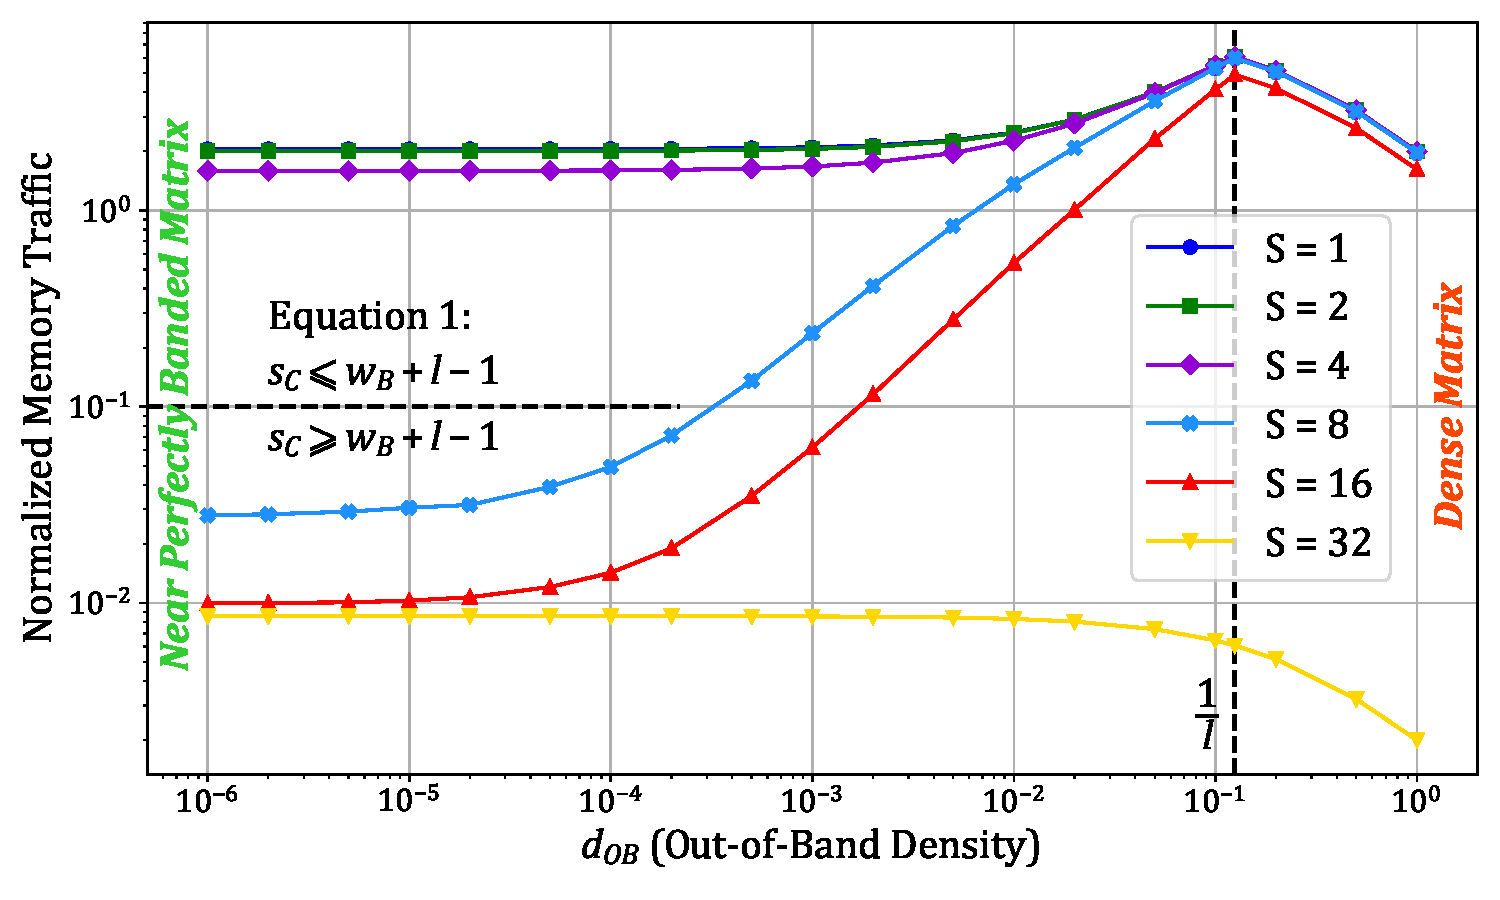
\includegraphics[width=\linewidth]{Chapter_Theory/Figures/PDF/graph1_25.07.31.pdf}
    \caption{Normalized Output Memory Traffic Depending on the Out-of-\Gls{band} Density for Several Cache-Sizes}
    \label{fig:theory:theory_traffic_vs_d_ob}
\end{figure}

On the right of the graph, we notice that $\mathit{normMT}$ reaches a peak when the out-of-\gls{band} density equals \mbox{$\frac{1}{l} = 0.125$}.
Indeed, when there is at least one non-zero element per cache-line, the behavior of the cache approaches that seen for a dense matrix.
As the density increases further, the traffic remains constant, thus $\mathit{normMT}$ drops, as seen in the graph in Figure~\ref{fig:theory:theory_traffic_vs_d_ob}

For the plot corresponding to $S = 32$, the cache is large enough to store the entire output vector $c$, thus, there are no \glspl{eviction} and $\mathit{normMT}$ is constant, corresponding to the flush traffic at the end.
This plot gives the lower bound of memory traffic for the output vector $c$.

The first takeaway of this graph is that variations in $d_\mathit{OB}$ heavily impact $\mathit{normMT}$.
Isolated non-zero elements outside the \gls{band} trigger misses and \glspl{eviction} of cache-lines corresponding to the \gls{banded} region.
Furthermore, when a cache-line is allocated for an isolated out-of-\gls{band} element, most of the cache-line remains empty.
In this case, instead of the efficient rotating pattern described in Section~\ref{sec:perfectband_vs_cache}, the cache is \textit{thrashing} with low utilisation.
Regardless of the cache-size, the lower the out-of-\gls{band} density, the lower $\mathit{normMT}$, as seen by the plots that tend downward toward the left of the graph.
Avoiding the perturbations induced by the out-of-\gls{band} elements would enable the cache to achieve minimal memory traffic, as with a \gls{PBanded} matrix.

Not surprisingly, at the left of the graph, $\mathit{normMT}$ varies depending on the cache-size.
This is due to the relative size of the \gls{band} and the cache.
Indeed, if the matrix \gls{band} width is large compared to the cache-size, processing one column of the \gls{band} will generate many \glspl{eviction}.
To avoid \glspl{eviction} in the \gls{band}, the relationship given by Equation~\ref{eq:theory:in_band_cond} in Section~\ref{sec:perfectband_vs_cache} must be fulfilled.
Indeed, for this example, for $S \geqslant 8$, this relationship holds and the corresponding plots have significantly lower $\mathit{normMT}$.
Conversely, the first three plots ($S = 1$ to $4$) do not respect this condition, explaining their high $\mathit{normMT}$.
Thus, the second takeaway from this graph is that, given a cache memory size, there is an ideal \gls{band} width that generates minimal $\mathit{normMT}$.
Increasing the cache-size beyond this threshold only produces a minor reduction in memory traffic, since at the beginning of matrix traversal, the first \gls{eviction} is deferred before reaching the steady state rotating pattern, as discuss in Section~\ref{sec:perfectband_vs_cache}.

These observations lead us to divide the cache into two regions.
One which is optimized for storing the \gls{band} and the other which handles all the other elements.
The in-\gls{band} region of the cache can thus operate with maximal efficiency corresponding to the bottom-left of Figure~\ref{fig:theory:theory_traffic_vs_d_ob}.
In subsequent sections, we analyse the out-of-\gls{band} traffic.

% %%%%%%%%%%%%%%%%%%%%%%%%%%%%%%%%%%%%%%%%%%%%%%%%%%%%%%%%%%%%%%%%%%%%%
\subsection{Design Analysis for Out-of-Band Region}
\label{sec:graph2}

For the type of large matrices under study, there are usually too many non-zero elements in the out-of-\gls{band} region for them to be cached from one column to the next, thus making it impossible to achieve the rotating pattern described in Section~\ref{sec:perfectband_vs_cache}.
Therefore, the size of the cache for the out-of-\gls{band} is not as important as the choice of associativity and data granularity.
To justify this affirmation, we use the analytical model from Section~\ref{sec:theory:model} to analyse the performance of the \gls{redC} when processing only the non-zero elements outside of the \gls{band}.
As we have already discussed the handling of the in-\gls{band} region, we now consider only the out-of-\gls{band} elements, which is equivalent to setting the in-\gls{band} density to $d_\mathit{IB} = 0$.
Using the same matrix parameters as in the previous section, we explore different choices of cache-line size ($l \in \{1, 8\}$ elements), associativity (set-associative or fully-associative), memory transaction type (\textit{R/W} or \textit{RMW}), and total cache-size ($s_C \in \{128, 256\}$ elements).
Because the out-of-\gls{band} data is highly sparse, we want to explore having an element-wise cache ($l = 1$) instead of the typical line-wise cache ($l = 8$).
As this cache region can be relatively small, a fully-associative configuration ($S = 1$, $l = 1$) is reasonable in terms of hardware implementation, and this full associativity makes full use of the storage.
Indeed, when dealing with sparse elements, it is wasteful to bring a full line into the cache to only modify one element and then evict it, which we denote as \textit{R/W}.
Thus, we consider offloading the \textit{reduction} to a higher level cache, thus reducing unnecessary data transfers.
We assume the higher level cache can support this operation which we denote as \textit{RMW}.
Indeed, protocols such as AXI~\cite{ARM2023_AXI} support atomic transactions (AMOs), which could easily be extended for \textit{reduction} operations.

To validate that the cache-size is of secondary importance, we consider two different sizes (\textit{solid} and \textit{dashed}).
For a given cache-size, we adjust the number of ways ($W$), based on the associativity, to keep the cache-size constant.
In Figure~\ref{fig:theory:theory_OBtraffic_vs_d_OB}, we plot $\mathit{normMT}$ for the output vector, depending on $d_\mathit{OB}$, for varying cache configurations.

\begin{figure}[htbp]
    \centering
    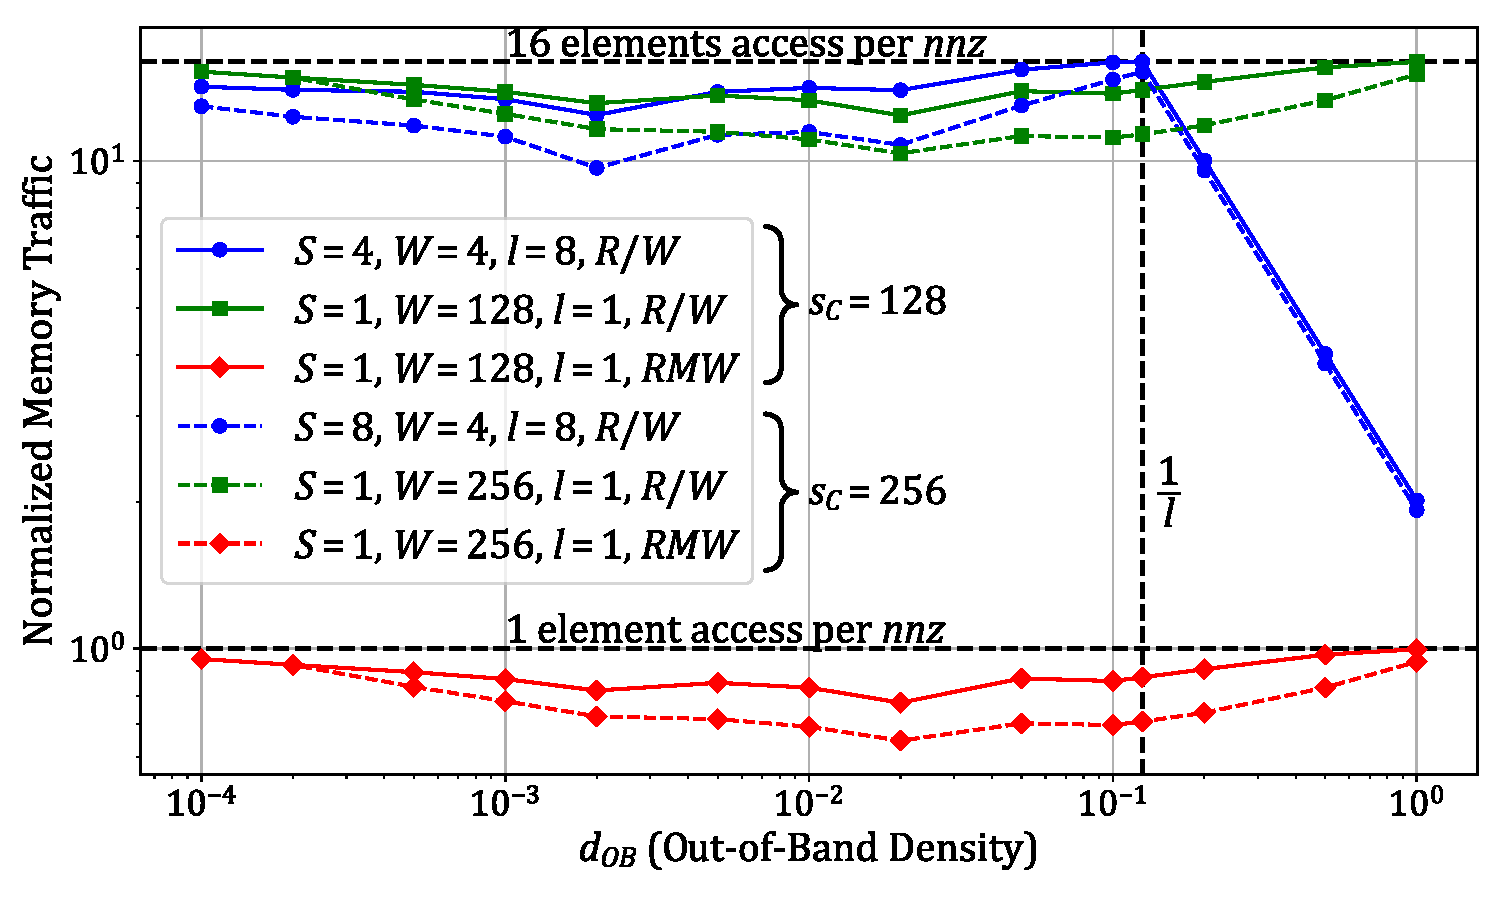
\includegraphics[width=\linewidth]{Chapter_Theory/Figures/PDF/graph3_25.07.31_modif.pdf}
    \caption{Normalized Output Memory Traffic of the Out-of-\Gls{band}, Depending on the Density for Several Cache-Sizes}
    \label{fig:theory:theory_OBtraffic_vs_d_OB}
\end{figure}

Let us start by considering a classic set-associative cache with a line-wise memory interface (\textit{solid blue}, \textit{dot}), where we see a dependence of $\mathit{normMT}$ on $d_\mathit{OB}$.
On the right of the graph ($d_\mathit{OB} \geqslant \frac{1}{l}$), we observe the same behavior as in Section~\ref{sec:graph1}, where the cache behavior approaches that seen for a dense matrix, where the cache tends to \textit{thrash}.

Looking at the plot for the fully-associative cache with a line-wise memory interface (\textit{solid green}, \textit{square}), we see that the normalized traffic is not impacted by the density of the out-of-\gls{band}, as expected.
With the fully-associative cache, $\mathit{normMT}$ is constant near $16$, as, on average, there are two line-wise transactions per non-zero element processed, one read to fill the line, one write to evict it.

The \textit{red} plots (\textit{diamond}) correspond to a fully-associative cache with an element-wise memory interface, which can offload element-wise \textit{RMW} transactions.
We see that this approach results in over an order magnitude reduction in $\mathit{normMT}$.
First, we avoid transferring full cache-lines which are mostly empty, and we only send the \textit{RMW} in one direction (``fire-and-forget'').
Indeed, $\mathit{normMT}$ is now reduced to below one transaction per non-zero element processed.
The fact that this value is below one shows that this cache region does hit and reduce memory traffic.
However, increasing the size of this cache does not significantly increase the hit-rate, as can be seen by the \textit{dashed} plots, which correspond to a $2\times$ larger cache, and which are not significantly lower than the corresponding \textit{solid} ones.

To summarize, the characteristics needed for the out-of-\gls{band} region are: (1) a fully-associative element-wise data-storage to avoid virtually empty cache-lines, (2) an element-wise memory interface to reduce memory traffic, and (3) a small storage region which is adequate.

% %%%%%%%%%%%%%%%%%%%%%%%%%%%%%%%%%%%%%%%%%%%%%%%%%%%%%%%%%%%%%%%%%%%%%
\subsection{Resulting Approach and Discussion}
\label{sec:theory_conclu}

In the previous sections, we analyzed the behavior of \textit{reduction caches} executing an \acrshort{op} \acrshort{spmv} kernel with \gls{banded} matrices.
We evaluated the expected memory traffic using an analytical model, considering separately the in- and out-of-\gls{band} regions.
We identified the cache characteristics required for both regions, which are extremely different.
We thus propose to divide the available cache memory into two dedicated regions: one for the in-\gls{band}, and one for the out-of-\gls{band}.

To obtain the efficient rotating pattern for the in-\gls{band} region, which is the key to massively reducing memory traffic, Equation~\ref{eq:theory:in_band_cond} must be respected.
In practice, this defines the size of the \gls{band} that can be allocated to the in-\gls{band} cache region.
As we have seen, this cache region can operate efficiently with a set-associative line-wise configuration.

For the out-of-\gls{band} region, a fully-associative element-wise cache with an element-wise memory interface can significantly reduce the memory traffic.
The size of this region is less critical, thus it is preferable to allocate the majority of the available storage to the in-\gls{band} region.

It is important to note that the analytical model that we have presented is based on the assumption of a uniform distribution of the non-zero elements.
In practice, this is not always the case, and this non-uniformity can impact the cache behavior, as will be seen later in Section~\ref{sec:evaluation}.
Indeed, if the non-zero elements are clumped, the cache-lines tend to be better filled, resulting in lower memory traffic.
In other words, our uniform assumption leads to a pessimistic prediction of memory traffic.